\documentclass[12pt]{article}

\usepackage[T2A]{fontenc}
\usepackage[utf8]{inputenc}
\usepackage[russian]{babel}

\usepackage{mathtext}
\usepackage{cmap}
\usepackage{amsmath,amssymb,amsthm,amscd,amsfonts}
\usepackage{graphicx}
\usepackage[colorbox,usenames,dvipsnames]{xcolor}
\usepackage{float, caption, subcaption, multirow}
\usepackage[section]{minted}
\usepackage{hyperref}
\usepackage{bbm}

\voffset -24.5mm
\hoffset -5mm
\textwidth 173mm
\textheight 240mm
\oddsidemargin=0mm \evensidemargin=0mm

\definecolor{codegray}{gray}{0.9}
\newcommand{\code}[1]{\colorbox{codegray}{\texttt{#1}}}
\newmintinline[src]{console}{}
\newmintinline[sql]{sql}{}

\renewcommand{\theFancyVerbLine}{\sffamily\textcolor{black}{\scriptsize\oldstylenums{\arabic{FancyVerbLine}}}}
\usemintedstyle[console]{bw}
\setminted[console] {
     bgcolor = codegray,
     linenos = true,
     tabsize = 2,
     formatcom = \color{black},
     frame = leftline,
     framerule = 0.8pt,
     framesep = 0.5cm,
     xleftmargin = 1cm,
     breaklines = true,
     escapeinside=||
}

\setminted[sql] {
     bgcolor = codegray,
     linenos = true,
     tabsize = 2,
     formatcom = \color{black},
     frame = leftline,
     framerule = 0.8pt,
     framesep = 0.5cm,
     xleftmargin = 1cm,
     breaklines = true,
     escapeinside=||
}

\newcommand{\pcell}[2]{\parbox[c]{#1\textwidth}{\textbf{#2}}}

\begin{document}

\title{
    Отчет по курсовой работе \\ 
    Дисциплина \\ <<Моделирование вычислительных систем>>}
\author{Евгений Хандыго, гр. 53501/3}

\begin{titlepage}
 \centerline{\bf Санкт-Петербургский политехнический университет Петра Великого}
 \centerline{\bf Институт компьютерных наук и технологий}
 \centerline{\bf Кафедра компьютерных систем и программных технологий}
 \vskip 5cm
{\large \centerline{\bf Отчет по курсовой работе}
 \centerline{\it Дисциплина «Программное обеспечение распределенных вычислительных систем»}}
 \vskip 1cm
 {\Large {\bf
} }

\vskip 3.9cm 
\rightline{Работу выполнил студент группы 63501/3}
\vskip 0.1cm 
\rightline{\underline{\hspace{3.7cm}} \hspace{1.1cm} Хандыго Е.Д.}

\vspace{0.5cm}

\rightline{Работу приняла}
\vskip 0.1cm 
\rightline{\underline{\hspace{3.7cm}} \hspace{1.0cm} Стручков И.В.}

\vskip 5cm 
\centerline{Санкт-Петербург}

\centerline{2016 г.}

\end{titlepage}

\tableofcontents
\newpage

\section{Анализ задания}

В рамках данного курса необходимо разработать простое приложение, позволяющее продемонстрировать основные архитектурные принципы 
проектирования программного обеспечения с использованием технологии Enterprise Java Beans (EJB). В качестве системы рассмотрим систему 
управлению персоналом, позволяющую автоматизировать некоторые аспекты повседневной деятельности работников компании. На этапе проектирования 
такой системы были выделены следующие роли и их интересы:

\begin{itemize}
    \item Работник 
    \begin{itemize}
        \item Сообщать время своего отсутствия в офисе.
        \item Резервировать время отпуска. 
    \end{itemize}
    \item Менеджер
    \begin{itemize}
        \item Имеет те же интересы, что и работник.
        \item Одобрять/отклонять запросы закрепленных за ним работников.
        \item Выписывать премию любому закрепленному за ним работнику. 
    \end{itemize}
    \item Бухгалтер
    \begin{itemize}
        \item Имеет те же интересы, что и работник.
        \item Одобрять/отклонять премию, выписанную работнику, закрепленному за ним.
    \end{itemize}
\end{itemize}

Используя эти данные, построим модель вариантов использования системы в виде UML диаграмы, как показано на рисунке \ref{fig:01-use-case}. 
При этом в системе должны функционировать следующие бизнес процессы:

\begin{itemize}
    \item Запрос на предоставление отпуска:
    \begin{enumerate}
        \item Пользователь системы выбирает желаемый период отпуска.
        \item Если менеджер не имеет вышестоящего начальника, то запрос автоматически подтверждается системой. В противном случае см. 
            пункт \ref{itm:propose-vocation-bp-3}.
        \item \label{itm:propose-vocation-bp-3} Запрос поступает менеджеру, за которым закреплен работник.
        \item Менеджер принимает или отклоняет запрос пользователя на предоставление отпуска в указанный период.
        \item В случае утверждения отпуска, соответствующая запись появляется в рабочем плане работника.
    \end{enumerate}
    \item Премирование работника:
    \begin{enumerate}
        \item Менеджер формирует запрос на выплату премии работнику, который закреплен за ним.
        \item Запрос поступает бухгалтеру, за которым закреплен данный работник.
        \item Бухгалтер утверждает или отклоняет запрос на выплату премии.
        \item В случае утверждения премии, соответствующая запись появляется в списке премиальных выплат работника.
    \end{enumerate}
    \item Указание времени отсутствия:
    \begin{enumerate}
        \item Работник может указать период собственного отсутствия по какой-либо причине.
        \item Данное действие не требует подтверждения со стороны --- соответствующая запись сразу же размещается в рабочем плане работника.
        \item Работник может удалить любую такую запись из своего собственного рабочего плана.
    \end{enumerate}
\end{itemize}

\begin{figure}[H]
    \centering
    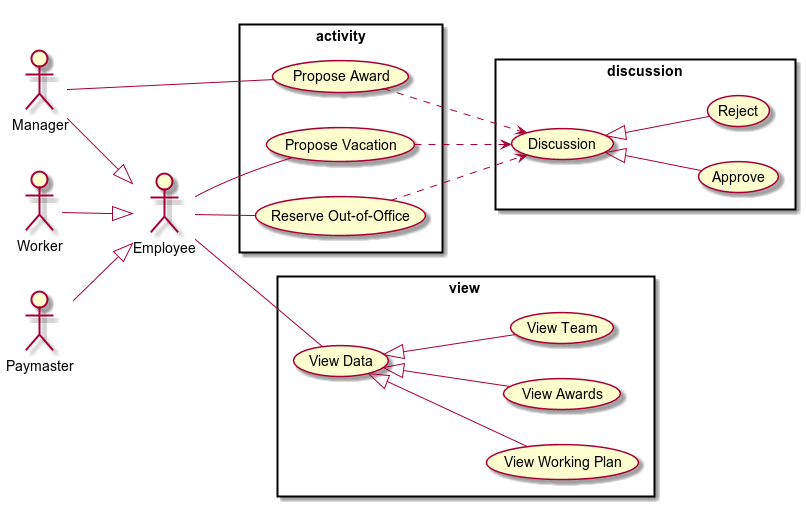
\includegraphics[width=\textwidth]{resources/01_analysis/01_use_cases.png}
    \caption{Диаграма вариантов использования системы}
    \label{fig:01-use-case}
\end{figure}

Приведем здесь подробный разбор вариантов использования системы:
\begin{itemize}
    \item Заявка на выделение премии:
    \begin{enumerate}
        \item \textbf{Пользователь}, выбирает сотрудника, которому необходимо выписать премию. 
        \item \textbf{Система} открывает форму премирования.
        \item \textbf{Пользователь} заполняет данную форму, указывая \textbf{когда} и в каком \textbf{размере} должна быть выплачена 
            премия.
        \item \textbf{Система} проверяет, что пользователь, отправивший заявку, действительно является менеджером по отношению к 
            премируемому сотруднику.
        \item В случае успеха \textbf{система} заносит запись о созданной заявке в базу данных.
        \item В случае ошибки на любом этапе \textbf{система} выводит сообщение об ошибке.
    \end{enumerate}
    \item Заявка на предоставление отпуска:
    \begin{enumerate}
        \item \textbf{Пользователь} нажимает кнопку.
        \item \textbf{Система} открывает форму заявки на предоставление отпуска.
        \item \textbf{Пользователь} заполняет форму.
        \item \textbf{Система} проверяет, что пользователь, отправивший заявку, соответствует работнику, на имя которого запрашивается 
            отпуск.
        \item В случае успеха \textbf{система} заносит запись о созданной заявке в базу данных.
        \item В случае ошибки на любом этапе \textbf{система} выводит сообщение об ошибке.
    \end{enumerate}
    \item Резервирование времени вне офиса:
    \begin{enumerate}
        \item \textbf{Пользователь} нажимает кнопку.
        \item \textbf{Система} открывает форму заявки на резервацию времени вне офиса.
        \item \textbf{Пользователь} заполняет форму.
        \item \textbf{Система} проверяет, что пользователь, отправивший заявку, соответствует работнику, на имя которого отправляется
            заявка.
        \item В случае успеха \textbf{система} заносит запись о созданной заявке в базу данных.
        \item В случае ошибки на любом этапе \textbf{система} выводит сообщение об ошибке. 
    \end{enumerate}
    \item Подтверждение заявки:
    \begin{enumerate}
        \item \textbf{Пользователь} нажимает кнопку.
        \item \textbf{Система} проверяет, что роль пользователя соответствует выполняемой операции:
        \begin{itemize}
            \item Если подтверждается заявка на премию, то пользователь должен иметь роль <<бухгалтер>>.
            \item Если подтверждается заявка на предоставление отпуска, то пользователь должен иметь роль <<менеджер>>.
        \end{itemize}
        \item В случае успеха \textbf{система} обновляет запись о соответствующей заявке в базу данных.
        \item В случае ошибки на любом этапе \textbf{система} выводит сообщение об ошибке. 
    \end{enumerate}
    \item Отклонение заявки:
    \begin{enumerate}
        \item \textbf{Пользователь} нажимает кнопку.
        \item \textbf{Система} проверяет, что роль пользователя соответствует выполняемой операции:
        \begin{itemize}
            \item Если отклоняется заявка на премию, то пользователь должен иметь роль <<бухгалтер>>.
            \item Если отклоняется заявка на предоставление отпуска, то пользователь должен иметь роль <<менеджер>>.
        \end{itemize}
        \item В случае успеха \textbf{система} обновляет запись о соответствующей заявке в базу данных.
        \item В случае ошибки на любом этапе \textbf{система} выводит сообщение об ошибке. 
    \end{enumerate}
\end{itemize}

Доменная модель системы в нашем случае описывается сущностями, представляющими пользователей системы и сущности, с которыми они 
взаимодействуют. Таким образом, модель предметной области в нотации UML будет выглядеть как показано на рисунке \ref{fig:01-domain}.

\begin{figure}[H]
    \centering
    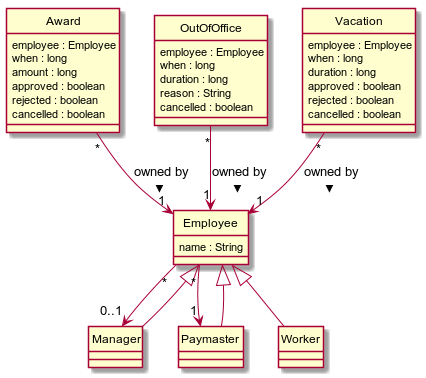
\includegraphics[width=0.8\textwidth]{resources/01_analysis/02_domain.png}
    \caption{Модель предметной области системы}
    \label{fig:01-domain}
\end{figure}


\section{Реализация}

\subsection{Объектно-ориентированное проектирование}

Перед началом реализации необходимо провести объектно-ориентированное проектирование системы. Данный этап подразумевает представление бизнес
логики в виде программных функций и разнесение этих функций по классам. Таким образом в программе формируется слой бизнес-логики. В данной 
случае этот слой было решено реализовать в виде набора сервисов. Наполнение классов осуществлялось так, чтобы соблюдались основные
принципы проектирования, такие, например, как принцип единственной ответственности (single responsibility principle). Результаты 
проектирования представлены ниже, на рисунке \ref{fig:02-bl} в виде UML диаграмы. 

\begin{figure}[H]
    \centering
    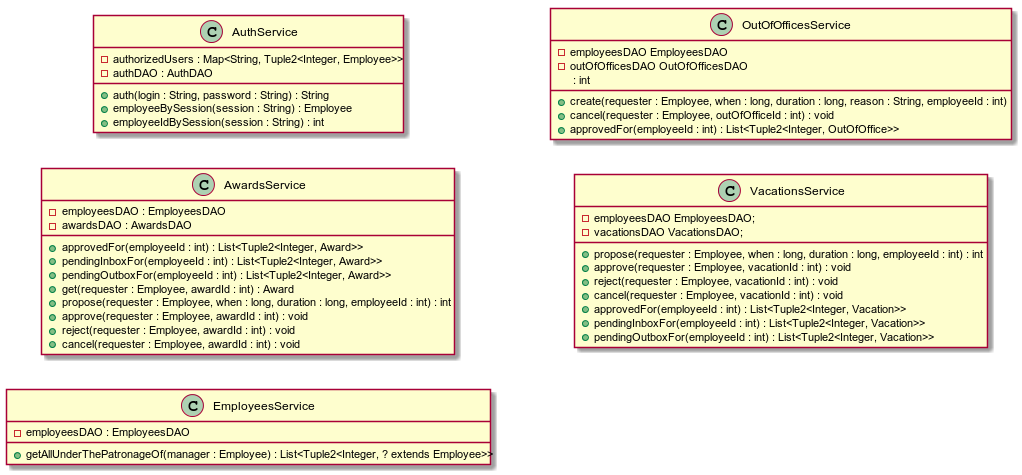
\includegraphics[width=\textwidth]{resources/02_implementation/01_bl.png}
    \caption{Модель предметной области системы}
    \label{fig:02-bl}
\end{figure}

Как видно, в результате проектирования было выделено $5$ сервисов. Каждый из классов параметризуется только лишь объектами доступа к данным
(DAO --- data access object) соответствующего типа. Приведем краткий разбор данных классов:

\begin{itemize}
    \item \code{AuthService} отвечает за авторизацию и аутентификацию пользователей, а также за выделение им специальных сессионных ключей.
    \begin{itemize}
        \item Процедура \code{auth} отвечает за выделение и сохранение сессионного ключа пользователю с заданными логином и паролем.
        \item Процедура \code{employeeBySession} отвечает за выдачу сущности пользователя по сессионному ключу.
        \item Процедура \code{employeeIdBySession} отвечает за выдачу идентификационного номера сущности пользователя по сессионному ключу.
    \end{itemize}
    \item \code{AwardsService} предназначен для работы с премиями.
    \begin{itemize}
        \item Процедура \code{approvedFor} предназначена для выдачи премий заданного пользователя, которые уже были подтверждены 
            бухгалтером. 
        \item Процедура \code{pendingInboxFor} предназначена для выдачи запросов на выплату премий, направленных заданному пользователю с
            ролью <<бухгалтер>>.
        \item Процедура \code{pendingOutboxFor} предназначена для для выдачи запросов на выплату премий, отправленных заданным 
            пользователем с ролью <<менеджер>>. 
        \item Процедура \code{get} выдает сущность-премию по ее идентификационному номеру. При этом осуществляется проверка прав доступа
            пользователя \code{requester} на доступ к заданной сущности.
        \item Процедура \code{propose} предназначена для создания запроса на выдачу премии заданному пользователю в заданный срок и с 
            заданным размером. При этом осуществляется проверка прав доступа пользователя \code{requester} на создание такого запроса с 
            указанным получателем.
        \item Процедура \code{approve} предназначена для подтверждения заданного запроса на выдачу премии. При этом осуществляется проверка 
            прав доступа пользователя \code{requester} на выполнение данного действия.
        \item Процедура \code{reject} предназначена для отклонения заданного запроса на выдачу премии. При этом осуществляется проверка 
            прав доступа пользователя \code{requester} на выполнение данного действия.
        \item Процедура \code{cancel} отменяет запрос на выдачу премий, который еще не был ни подтвержден, ни отклонен. При этом     
            осуществляется проверка прав доступа пользователя \code{requester} на выполнение данного действия.
    \end{itemize}
    \item \code{OutOfOfficeService} предназначен для работы с отсутствиями на рабочем месте.
    \begin{itemize}
        \item Процедура \code{create} предназначена для резервирования времени отсутствия в офисе в заданный период и с указанной причиной.
            При этом осуществляется проверка прав доступа пользователя \code{requester} на создание такого запроса с указанным получателем.
        \item Процедура \code{cancel} предназначена для отмены резервации времени нахождения вне офиса. При этом осуществляется проверка 
            прав доступа пользователя \code{requester} на выполнение данного действия.
        \item Процедура \code{approvedFor} предназначена для извлечения всех резерваций времени на отсутствие в офисе для указанного 
            пользователя.
    \end{itemize}
    \item \code{VocationService} предназначен для работы с отпусками. Здесь мы не будем приводить более подробный разбор методов данного 
        класса, поскольку все они аналогичны уже рассмотренным методам из класса \code{AwardsService}.
    \item EmployeeService отвечает за работу с пользователями.
    \begin{itemize}
        \item Процедура \code{getAllUnderThePatronageOf} отвечает за выдачу пользователей, которые подотчетны указанному пользователю.
    \end{itemize}
\end{itemize}

Также в рамках этапе объектно-ориентированного проектирования был создан набор диаграмм последовательностей в нотации UML (sequence duagram).
Ниже, на рисунках \ref{fig:02-propose-award} -- \ref{fig:02-decline-award} представлено несколько таких диаграмм для операций создания,
подтверждения и отклонения заявки на выдачу премии соответственно.

\begin{figure}[H]
    \centering
    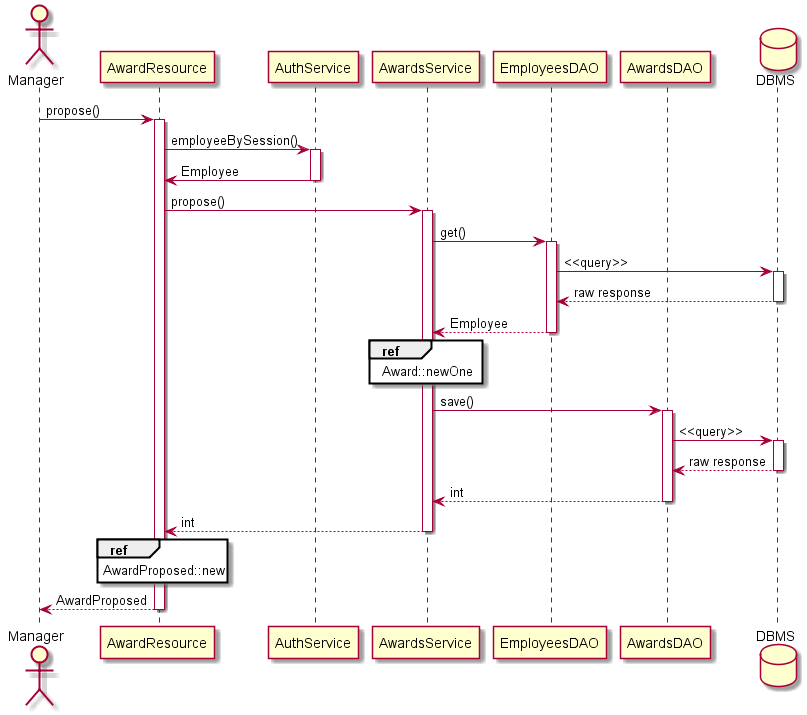
\includegraphics[width=\textwidth]{resources/02_implementation/02_award_employee.png}
    \caption{Процесс создания заявки на премирование}
    \label{fig:02-propose-award}
\end{figure}

\begin{figure}[H]
    \centering
    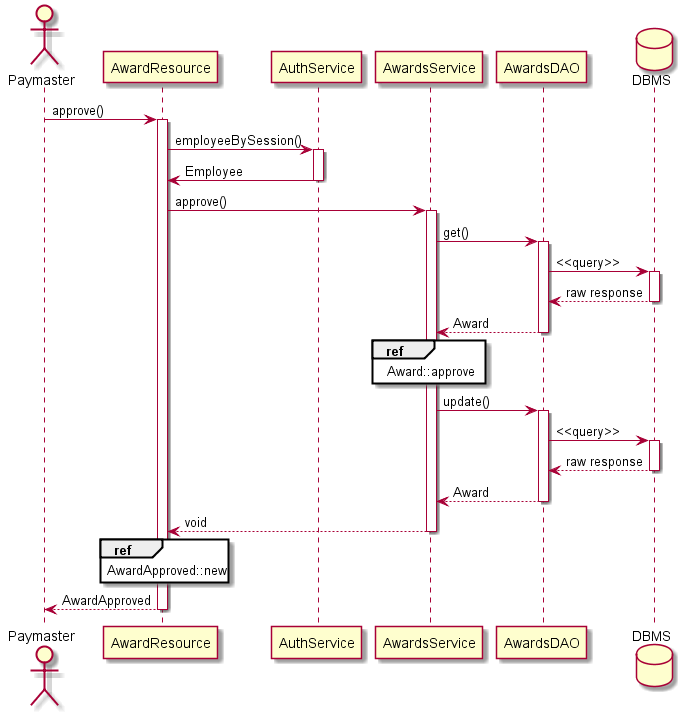
\includegraphics[width=0.55\textwidth]{resources/02_implementation/03_accept_award.png}
    \caption{Процесс подтверждения заявки на премирование}
    \label{fig:02-accept-award}
\end{figure}

\begin{figure}[H]
    \centering
    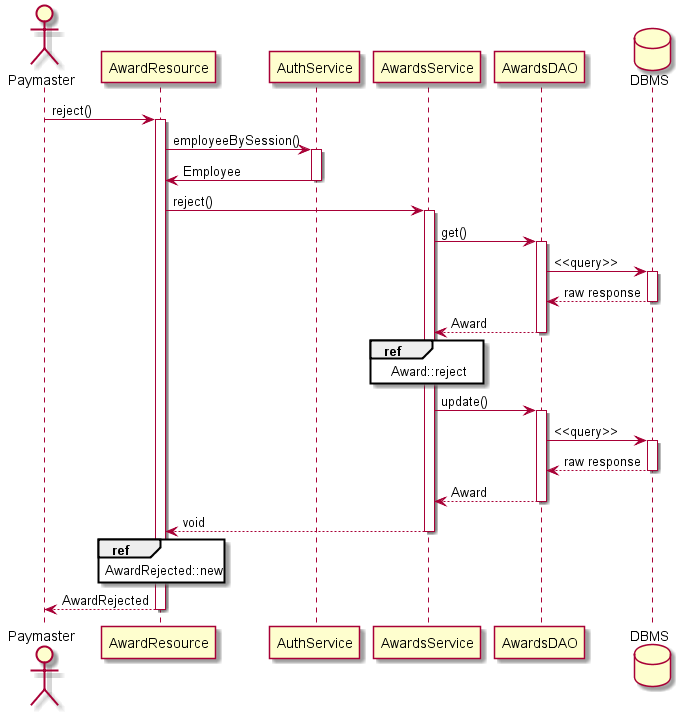
\includegraphics[width=0.55\textwidth]{resources/02_implementation/04_decline_award.png}
    \caption{Процесс отклонения заявки на премирование}
    \label{fig:02-decline-award}
\end{figure}

\subsection{Детали реализации}

Разработанное приложение необходимо реализовать в виде сетевого (web based) приложения. По этой причине, помимо уровня бизнес логики был 
также выделен уровень представления приложения, отвечающий за принятие запросов от клиента и отправку ему ответов. Методы, реализуемые на 
данном уровне, работают почти одинаково по следующей схеме:
\begin{itemize}
    \item Аутентификация пользователя путем обращения к экземпляру класса \code{AuthService}.
    \item Преобразование аргументов сетевого запроса к виду, удобному для уровня бизнес логики.
    \item Преобразованный запрос направляется на уровень бизнес логики, в соответствующий сервис.
    \item Результат, полученный от сервиса преобразуется к виду, удобному для ответа клиенту. 
\end{itemize}
Такая логика работы позволяет обеспечить независимость уровня бизнес логики от уровня представлений и, как следствие, большую гибкость. 
Другими словами, сервисные классы не имеют понятия о том, что приложение является сетевым, что позволяет переиспользовать данный код
при разработке, например, обычного (desktop) приложения. В то же время, любые изменения на уровне представления не затрагивают сервисный
уровень и, следовательно, не могут его <<сломать>>. Классы на уровне представления реализованы с учетом методики REST. Данный 
предоставляются в формате json. Преобразование объектов в формат json осуществляется при помощи библиотеки \code{jackson}. 

Из рисунка \ref{fig:02-bl} видно, что на уровне бизнес логики используются специальный объекты доступа к данным. Данные объекты также 
располагаются на отдельном уровне приложения --- уровне доступа к данным. Принцип работы методов, расположенных на данном уровне, совпадает
с логикой работы методов на уровне представления с той лишь только разницей, что здесь опускается этап аутентификации пользователей. 
Таким образом, обеспечивается такая же гибкость взаимоотношения между уровнями бизнес логики и доступа к данным, как и в случае уровней
представления данных и бизнес логики. Для реализации данного уровня использовалась библиотека \code{ebean-orm}, осуществляющая 
преобразование сущностей базы данных в программные сущности (object relational mapping). 

Также стоит отметить, что для избежания различных проблем, связанных с проектирование программного обеспечения, и для обеспечения 
гибкости в ходе реализации приложения была использована библиотека, осуществляющая внедрение зависимостей (dependency injection), --- 
\code{Guice}. Также для борьбы с кончервативным кодом (boilerplate code) была использована библиотека \code{lombok}.

\subsection{Методика и результаты тестирования}

На этапе тестирования использовались библиотеки \code{junit} и \code{mockito}. Использование данных библиотек позволило реализовать тесты
в соответствии с лучшими практиками. Отметим, что тестирование проводилось только для уровня бизнес логики. В силу большого количества
тестов и проверяемых в них условиях в рамках данной работы не будет приводиться сколь-нибудь подробное описание тестовых методов. Вместо
этого представим отчет по тестированию, сгенерированные при помощи утилиты \code{maven} и интегрированной среды разработки 
\code{IntelliJ IDEA}.

\begin{center}
    \inputminted{console}{resources/02_implementation/05_tests}
    \captionof{listing}{Отчет по тестированию, сгенерированный в \code{maven}}
\end{center}

\begin{figure}[H]
    \centering
    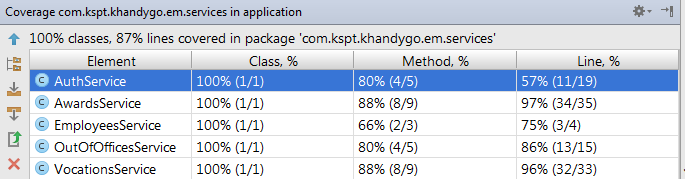
\includegraphics[width=\textwidth]{resources/02_implementation/06_tests.png}
    \caption{Отчет по тестированию, сгенерированный в \code{IntelliJ IDEA}}
    \label{fig:02-test}
\end{figure}

\subsection{Инструкция системного администратора}

Для развертывания приложения необходимы следующие системные компоненты:
\begin{itemize}
    \item Сервер \code{MySQL} версии $5.5$ или выше.
    \item Утилита \code{maven} версии $3.1.0$ или выше.
    \item Сервер приложений \code{wildfly} версии $10.1.0$ или выше.
\end{itemize}
Теперь необходимо настроить \code{MySQL} сервер следующим образом:
\begin{itemize}
    \item Порт $3307$.
    \item Создать схему с именем \code{test}.
    \item Наполнить базу данных так, как показано в листинге \ref{lst:02-mysql-create}. 
    \item Создать пользователя с логином \code{em\_admin} и паролем \code{1234}.
    \item Выделить пользователю \code{em\_admin} права на чтение и запись в схеме \code{test}.
\end{itemize}
Никакой дополнительной настройки \code{maven} и \code{wildfly} не требуется. Для запуска сервера приложений в простейшем случае можно
воспользоваться скриптом \code{standalone} (расширение \code{.bat} или \code{.sh} зависит от используемой операционной системы и средств),
расположенным в директории \code{bin}. Теперь для размещения проекта на сервере необходимо выполнить команду \code{mvn clean install 
wildfly:deploy} из директории проекта. Здесь, конечно, предполагается, что на рабочей машине есть доступ к сети Интернет.

\begin{center}
    \inputminted[lastline=34]{sql}{resources/02_implementation/07_mysql_create}
    \inputminted[firstline=35]{sql}{resources/02_implementation/07_mysql_create}
    \captionof{listing}{Скрипт создания базы данных приложения \label{lst:02-mysql-create}}
\end{center}

Для создания пользователя системы необходимо выполнить в \code{MySQL} команду вида
\begin{center}
    \sql{INSERT INTO users VALUES(null, login, MD5(pswd), name, m_id, p_id);},
\end{center}
где: \code{login} --- логин пользователя, \code{pswd} --- пароль пользователя, \code{name} --- имя пользователя, \code{m\_id} и 
\code{p\_id} --- идентификационные номера менеджера и бухгалтера данного пользователя соответственно. 

В случае правильной настройки всех компонент приложение должно быть доступно по адресу сервера приложений на порте с номером $8080$
с добавлением \code{/application}.

\subsection{Инструкция пользователя}

Для того, чтобы начать пользоваться системой необходимо сначала пройти аутентификацию на заглавной странице. Для этого в соответствующие 
поля вводятся логин и пароль пользователя. Далее, в левой части экрана будет доступно меню. 
\begin{itemize}
    \item Для того, чтобы просмотреть подтвержденные заявки на отпуск и выплату премии необходимо перейти по пункту \code{Home}.
    \item Для того, чтобы просмотреть информацию о своем менеджере и бухгалтере, необходимо перейти по пункту \code{Stuff}.
    \item Для того, чтобы просмотреть информацию об отправленных, но еще не подтвержденных и не отклоненных заявках, а также заявках,
        направленных данному пользователю, необходимо перейти по вкладке \code{Proposals}.
    \item Для того, чтобы отправить заявку на предоставление отпуска необходимо нажать кнопку \code{Propose Vacation}.
    \item Для того, чтобы зарезервировать время отсутствия в офисе необходимо нажать кнопку \code{Reserve Out Of Office}.
\end{itemize}

\section{Вывод}

В рамках данной работы было разработано и реализовано сетевое приложение на языке Java с использованием технологии EJB. Считаю, что приложение
разработано и реализовано на высоком уровне. Развитие приложения с функциональной точки зрения может быть продолжено в добавлении новых
бизнес процессов. С точки зрения развертывания, в первую очередь необходимо добавить возможность конфигурации приложения из конфигурационного
файла. В данном случае этого не было сделано по причине специфики работы выбранного сервера приложений с ресурсными файлами.

Дадим оценку приложения с точки зрения различных характеристик распределенных систем:
\begin{itemize}
    \item \textbf{Прозрачность} обеспечивается методикой REST на уровне представления приложения. 
    \item \textbf{Открытость} достигается тем, что приложение обладает сетевым интерфейсом. 
    \item \textbf{Масштабируемость} приложения оценить достаточно сложно. Можно только предположить, что достаточно разместить приложение 
        на распределенном сервере приложений.
\end{itemize} 

\end{document}